\section{Project Timeline}
This 36-month PhD research will progress through four key phases, with critical milestones at months 3 (M1: protocol finalization), 9 (M2: data acquisition completion), 18 (M3: vulnerability mapping), and 30 (M4: model validation), culminating in thesis submission at month 36. Figure \ref{fig:gantt} presents a detailed timeline of research activities including faculty assessment milestones.
\begin{figure}[h]
\centering
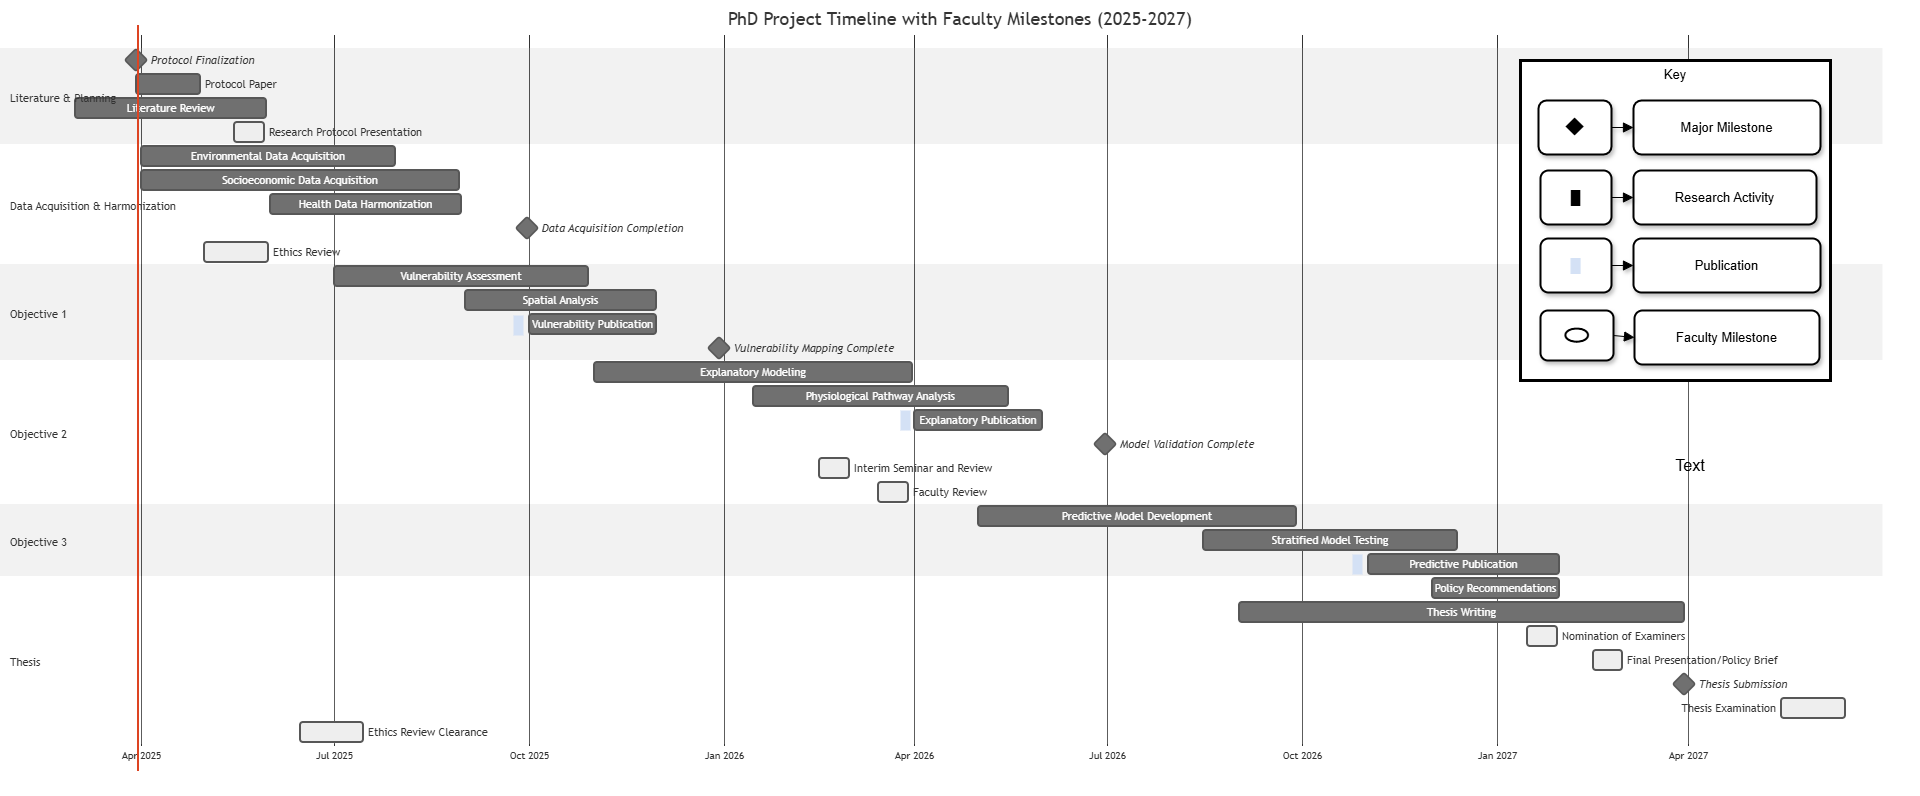
\includegraphics[width=0.95\textwidth]{sections/images/GANTT.png}
\caption{Project Timeline with Key Research Milestones and Publications}
\label{fig:gantt}
\end{figure}
The research timeline includes four major publications: a protocol paper titled ``Leveraging data science and machine learning for urban climate adaptation in two major African cities: a HE2AT Center study protocol'' \cite{Jack} (Month 4), followed by three objective-specific publications: ``Quantifying intra-urban socio-economic and environmental vulnerability to extreme heat events in Johannesburg, South Africa'' (Month 9), ``Uncovering Heat-Health Pathways in Johannesburg: An Explanatory Machine Learning Approach Using Harmonized Urban Cohort Data'' (Month 19), and ``Developing Stratified Heat-Health Early Warning Systems for Johannesburg: Integration of Vulnerability Mapping and Predictive Modeling'' (Month 33).
Primary risks include data accessibility challenges, computational constraints, and model performance issues. Detailed timelines, activities, and risk mitigation strategies are provided in Appendix C.